\begin{frame}
  \frametitle{\textbf{Quantum Chromodynamics}}
  \begin{columns}
    \column{0.6\textwidth}
    \begin{itemize}
    \item \textbf{Quantum chromodynamics} (QCD) is a quantum field theory describing the \textbf{strong interaction} between \textbf{quarks} and \textbf{gluons}
    \item \textbf{Confinement}: fundamental feature of QCD
      \begin{align*}
        V_{\text{QCD}}(Q^2) = \color{gray}\underbrace{\color{black}-\cfrac{4}{3}\cfrac{\alpha_s(Q^2)}{r}}_{\text{QED-like short-range}} \color{black} + \color{gray} \underbrace{\color{black}\lambda r}_{\text{QCD long-range}}
      \end{align*}
    \item QCD is a quantum field theory with \textbf{asymptotic freedom}
    \end{itemize}
    \begin{align*}
      &\alpha_s(Q^2) = \cfrac{\alpha_s(\mu^2)}{1 + \left[\alpha_s(\mu^2)\frac{(11n_c - 2n_f)}{12\pi}\right]\ln\left(\frac{Q^2}{\mu^2}\right)} \\
      & \boxed{\lim_{Q \to \infty}\alpha_s(Q^2) \to 0}
    \end{align*}

    \begin{itemize}
    \item Large $Q^2 \to$ strong-force coupling gets \textbf{weaker}
    \end{itemize}



    \column{0.4\textwidth}
    \centering
    \begin{tikzpicture}
      \node{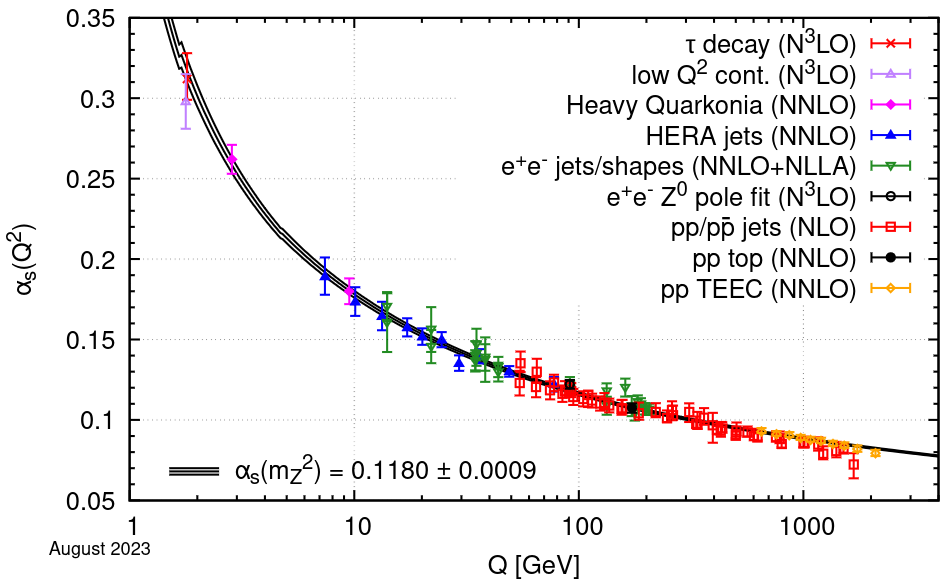
\includegraphics[width=0.9\textwidth]{running-coupling.png}};
      \node[font=\tiny,align=left] at (0.2,2.1) {\href{https://academic.oup.com/ptep/article/2022/8/083C01/6651666}{Prog. Theor. Exp. Phys. 2022, 083C01 (2022)}};
    \end{tikzpicture}

    \

    \

    \begin{columns}

      \column{0.33\textwidth}
      \resizebox{\textwidth}{\textwidth}{
        \begin{tikzpicture}
          \begin{feynman}
            \vertex (a) {\( q \)};
            \vertex[below right=of a] (b);
            \vertex[below left=of b] (c) {\( q \)};
            \vertex[right=of b] (d) {\( g \)};
            \diagram*{
              (a) -- [fermion] (b),
              (b) -- [fermion] (c),
              (b) -- [gluon] (d),
            };
          \end{feynman}
        \end{tikzpicture}
      }

      \column{0.33\textwidth}
      \resizebox{\textwidth}{\textwidth}{
        \begin{tikzpicture}
          \begin{feynman}
            \vertex (a) {\( g \)};
            \vertex[below right=of a] (b) ;
            \vertex[below left=of b] (c) {\( g \)};
            \vertex[right=of b] (d) {\( g \)};
            \diagram*{
              (a) -- [gluon] (b),
              (b) -- [gluon] (c),
              (b) -- [gluon] (d),
            };
          \end{feynman}
        \end{tikzpicture}
      }

      \column{0.33\textwidth}
      \resizebox{\textwidth}{\textwidth}{
        \begin{tikzpicture}
          \begin{feynman}
            \vertex (a) {\( g \)};
            \vertex[below right=of a] (b) ;
            \vertex[below left=of b] (c) {\( g \)};
            \vertex[above right=of b] (d) {\( g \)};
            \vertex[below right=of b] (e) {\( g \)};
            \diagram*{
              (a) -- [gluon] (b),
              (b) -- [gluon] (c),
              (b) -- [gluon] (d),
              (b) -- [gluon] (e),
            };
          \end{feynman}
        \end{tikzpicture}
      }

    \end{columns}
    

    
  \end{columns}
\end{frame}
